\newpage
\thispagestyle{empty}
\begin{center}
\vspace*{-0.5cm}
{\normalsize\textbf{DEPT. OF ELECTRONICS \& COMMUNICATION ENGINEERING}}\\[0.2cm]
{\normalsize\textbf{AMAL JYOTHI COLLEGE OF ENGINEERING (AUTONOMOUS)}}\\[0.2cm]
{\normalsize\textbf{KANJIRAPPALLY}}\\[0.5cm]
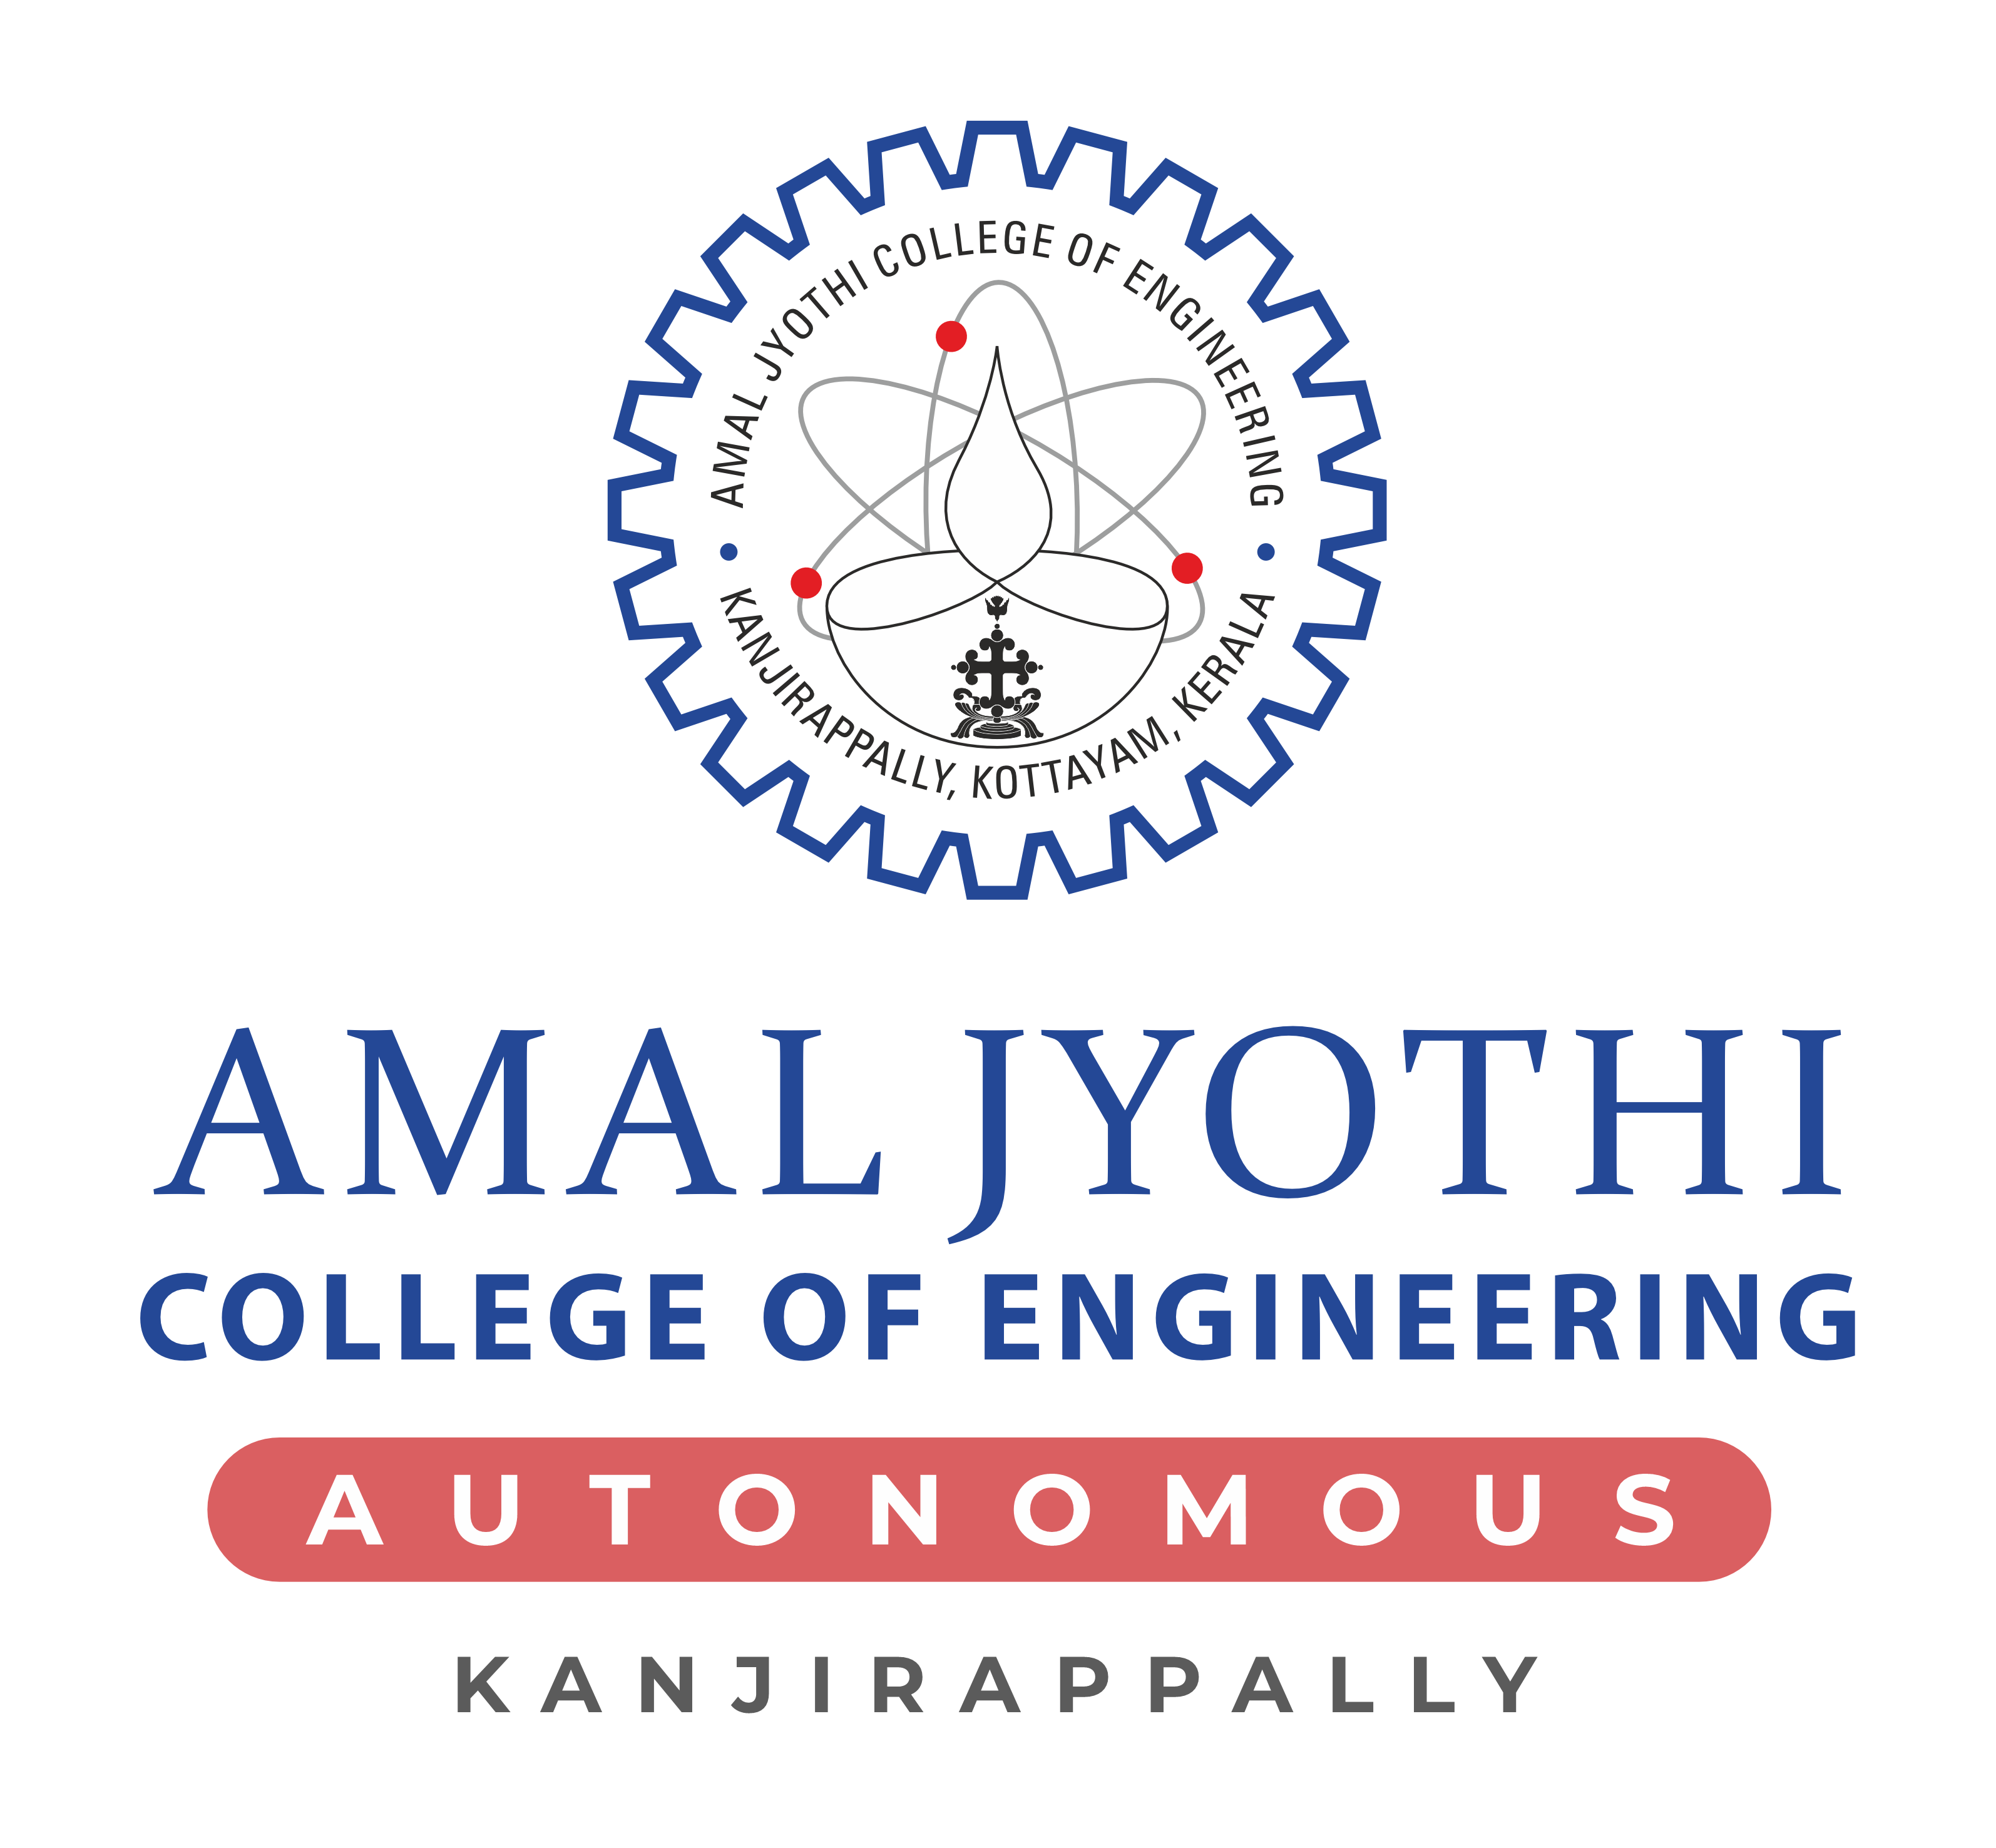
\includegraphics[width=0.22\textwidth]{assets/ajcelogo2023.png}\\[0.6cm]
{\Large\textbf{CERTIFICATE}}
\end{center}
\vspace{0.4cm}

\noindent
\begin{spacing}{1.5}
This is to certify that \textbf{Abin Varghese (AJC23CS008)}, \textbf{Alfin Shabu (AJC23CS012)}, \textbf{Alan Jimmy (AJC23CS010)}, and \textbf{Amith Mathew (AJC23CS015)} have satisfactorily completed their MINI PROJECT entitled ``\textbf{AI-Based Autonomous Navigation and Real-Time Collision Avoidance System for Micro-Vehicles}'' as a part of the partial fulfilment of the requirements for the award of the \textbf{MINOR in ELECTRONICS AND COMMUNICATION ENGINEERING} from Amal Jyothi College of Engineering, Kanjirappally, affiliated to APJ Abdul Kalam Technological University, Kerala.
\end{spacing}

\vspace{2.6cm}

\noindent
\begin{tabular*}{\textwidth}{@{}c@{\extracolsep{\fill}}c@{}}
\textbf{Mr. Binu Mathew} & \textbf{Dr. Gee Varghese Titus} \\
Internal Supervisor & Head of the Department, ECE
\end{tabular*}
